\documentclass{article}
\usepackage[utf8]{inputenc}
%\usepackage{multicol}
\usepackage{graphicx}
\usepackage{vmargin}
\usepackage{float}

\setpapersize{A4}
\setmargins{2.5cm}       % margen izquierdo
{1.5cm}                        % margen superior
{16.5cm}                      % anchura del texto
{23.42cm}                    % altura del texto
{10pt}                           % altura de los encabezados
{1cm}                           % espacio entre el texto y los encabezados
{0pt}                             % altura del pie de página
{2cm}                           % espacio entre el texto y el pie de página
\title{Tarea Metodos Computacionales}
\author{Alexander Sierra Pulido \thanks {a.sierra12@uniandes.edu.co} \\\textit{{Departamento de Fisica}}\\\textit{{Universidad de los Andes - Bogotá, Colombia }}}
\date{Jul 18, 2019}

\begin{document}

\maketitle
\hrulefill
\begin{abstract}

A continuación, se presentarán dos temas importantes dentro del curso de métodos computacionales, ofrecido por la universidad de Los Andes. El primero de estos es la transformada de Fourier, la cual es bastante útil a la hora de realizar filtros a imágenes o señales, aunque ya se ahondara en el tema. El segundo, aún más necesario para las ciencias e ingenierías, son las ecuaciones diferenciales ordinarias. Así que el siguiente texto está dividido en dos partes principales, donde cada una explicará brevemente la importancia del problema y su sentido físico; del mismo modo se mostraran los resultados obtenidos a partir de scripts de Python y C++.      

\end{abstract}
\hrulefill
%%%%%%%%%%%%INTRODUCCIÓN%%%%%%%%%%%%%%%%%%%%%%

\section{Transformada de Fourier en 2D}
Este reporte se enfocara en tan solo una de las diversas aplicaciones de la transformada de Fourier, el cual es la creación de imágenes híbridas a partir de filtros. Las imágenes híbridas son una técnica que produce imágenes estáticas con dos interpretaciones, dependiendo de la distancia a la que se observe. La idea de este ejercicio es hacer una imagen híbrida, explicando y mostrando su proceso de creación paso a paso, a partir de dos imágenes de una misma persona con dos expresiones faciales diferentes.\\ 

En primer lugar, lo que se debe hacer es leer las fotografías como un arreglo que contiene la información necesaria para realizar su transformada de Fourier. Una vez se ha realizado esta transformada de Fourier para cada una de las imágenes, el resultado es el siguiente. 

\begin{figure}[H]
    \centering
    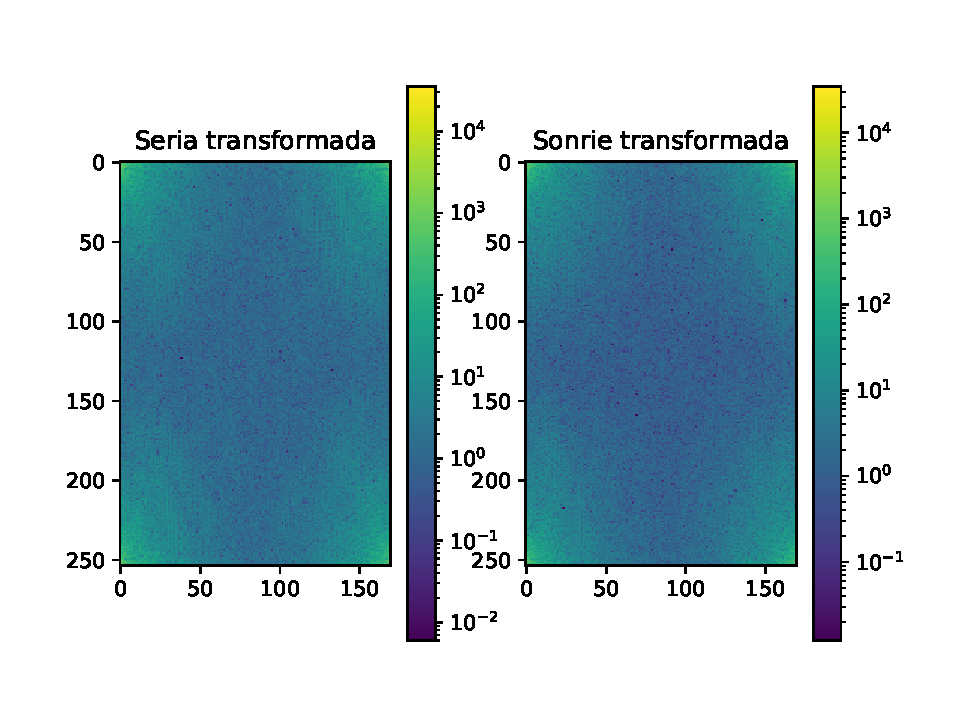
\includegraphics[width=\textwidth]{FFtIm.pdf}
    \caption{En la imagen se muestra el espectro de Fourier para cada una de las imagenes.}
    \label{fig:FFT}
\end{figure}

A continuación lo que se debe hacer, teniendo ya la figura\ref{fig:FFT}, es realizar el filtro. Este filtro es importante ya que en este radica gran parte de la clave de que la imagen híbrida salga bien. Entonces, lo ideal sería aplicar un filtro gaussiano a una imagen y a la otra un filtro pasa altos. En el desarrollo de este problema se decidió usar un filtro pasa bajos en vez de un desenfoque gaussiano, ya que para efectos prácticos funciona bastante bien. A continuación se muestra el proceso de filtros y cambio a un espacio de amplitudes. 

\begin{figure}[H]
    \centering
    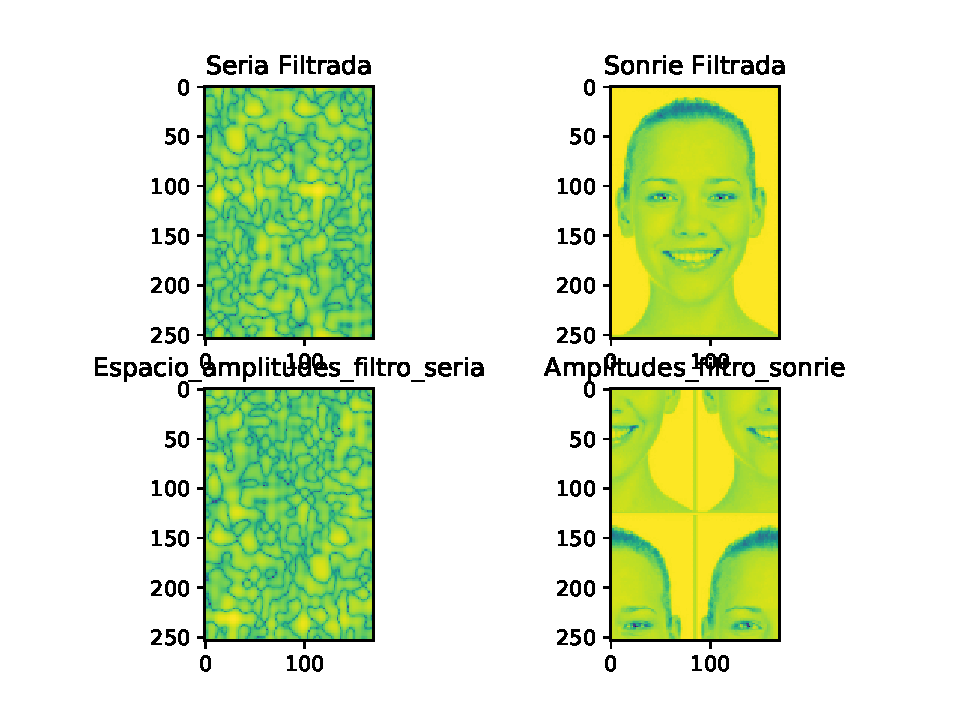
\includegraphics[width=\textwidth]{ImProceso.pdf}
    \caption{En la imagen se muestra en la parte de arriba lo que sucede despues de aplicar el filtro, mientras que en las imagenes de abajo se muestra lo que sucede cuando volvemos al espacio de amplitudes(estabamos en el espacio de frecuancias).}
    \label{fig:pro}
\end{figure}

Finalmente, luego de esto debemos sumar ambas imagenes (acá puede ser de utilidad multiplicar ambas imagenes por un numero entre 0 y 1) y aplicar la transformada inversa de la superposición de las imagenes. Lo cual nos permite observar el siguiente resultado:

\begin{figure}[H]
    \centering
    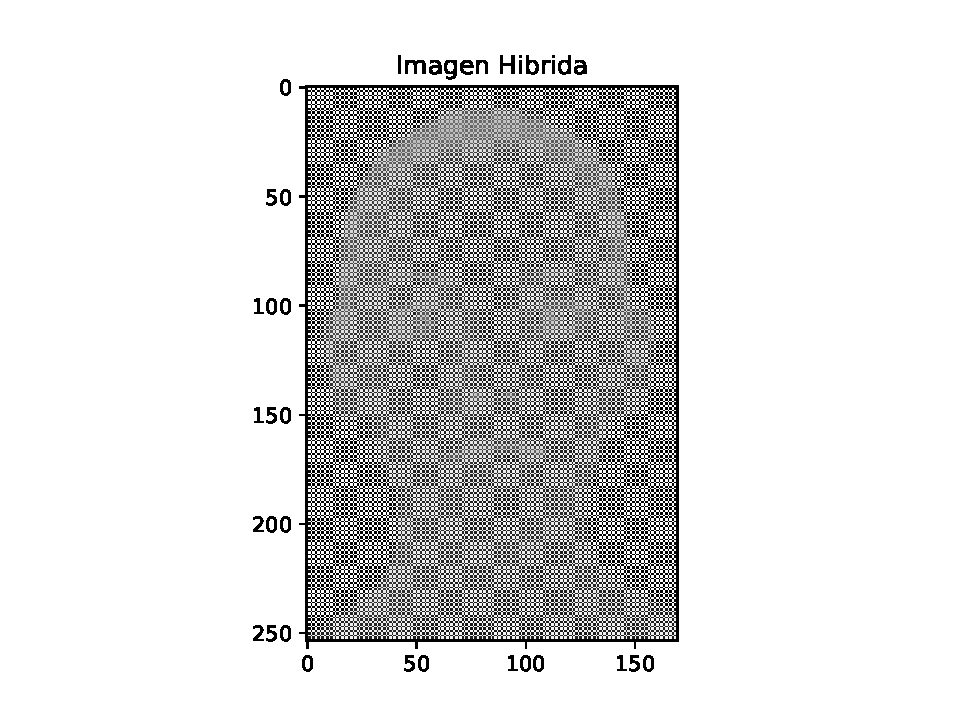
\includegraphics[width=\textwidth]{Hibrida.pdf}
    \caption{Se muestra la imagen híbrida obtenida del proceso anteriormente descrito.}
    \label{fig:hib}
\end{figure}

\section{Ecuaciones diferenciales ordinarias}
En este caso se evaluará el sistema tierra-sol, el cual se puede modelar mediante la siguiente ecuación diferencial: 

\begin{equation}
    \frac{d^{2}x(t)}{dt^{2}} = -G\frac{M_{sol}}{r_{12}^{3}}(r_{2}-r_{1})
\end{equation}

donde "G" es la constante universal de gravitación, y "r" la distancia entre ambos cuerpos. Teniendo esto en cuenta, se debe aclarar que como se solucionará el problema mediante métodos computacionales, el desarrollo del mismo difiere de métodos numéricos. Los métodos computacionales vistos en clase se diferencian entre si en la manera en como se calcula la derivada de las variables; en este caso: Euler usa forward difference, Leap-frog usa central difference, y Runge Kutta es un poco más complejo (y preciso) ya que usa varios puntos intermedios y constantes para hallar la derivada.\\

La idea de este ejercicio es comparar los métodos de Euler, Runge Kutta de 4to orden y LeapFrog, asumiendo que el movimiento del Sol es despreciable y que se puede considerar que este está fijo. Sin mucho mas preámbulo, se presentará la gráfica correspondiente a 20 orbitas para cada uno de los métodos nombrados, cambiando el parámetro dt. 


\begin{figure}[H]
    \centering
    \includegraphics[width=\textwidth]{XY_met_dt.pdf}
    \caption{En la imagen se observan 6 gráficas distintas. En los títulos de cada gráfica se menciona el dt usado. Finalmente, cada columna representa el mismo método, para que sea más sencillo su comparación.}
    \label{fig:pos}
\end{figure}

En la figura\ref{fig:pos}, se evidencia el dominio del método LeapFrog para conservar la misma orbita y no acercarse hacia el sol. Aunque los otros dos métodos no son incorrectos, podemos confirmar que LeapFrog es el que mejor funciona en el caso de la posición de la tierra en su orbita en el del tiempo.\\   

Por otra parte, además de calcular las posiciones durante el rango de tiempo, se calculó la velocidad en cada una de las coordenadas espaciales y, al igual que para el caso anterior, se procedió a realizar la gráfica lo sucedido para cada método y para cada dt.  

\begin{figure}[H]
    \centering
    \includegraphics[width=\textwidth]{VxVy_met_dt.pdf}
    \caption{En la imagen se muestran los resultados de calcular la velocidad en "x" y en "y". Evidentemente, las gráficas mejoran cuando el dt es más pequeño.}
    \label{fig:vel}
\end{figure}

Así, podemos observar que en la figura\ref{fig:vel} es sencillo diferenciar en que métodos se conserva de mejor manera la energía cinética. Aunque Runge Kutta suele ser el método mas preciso, ahora estamos viendo que LeapFrog conserva casi que perfectamente la energía cinética. Además, de nuevo se puede concluir que el método de Euler es más impreciso que los demás pero esto radica nuevamente en la definicion del mismo.\\

En adición a lo anterior, se presentarán dos análisis más con respecto al caso de estudio. El primero es el cálculo y resultados de la variación del momento angular con respecto al tiempo. El segundo es el análisis de la energía mecánica de la tierra durante su traslación. 

\begin{figure}[H]
    \centering
    \includegraphics[width=\textwidth]{Mome_met_dt.pdf}
    \caption{En la imagen se muestran los resultados de calcular el momento angular de la tierra en cada paso de tiempo.}
    \label{fig:Mome}
\end{figure}

\begin{figure}[H]
    \centering
    \includegraphics[width=\textwidth]{Ener_met_dt.pdf}
    \caption{En la figura se observa la variación de la energía mecánica de la tierra con respecto al tiempo los resultados de calcular la velocidad en "x" y en "y".}
    \label{fig:Ene}
\end{figure}
 
En la figura\ref{fig:Mome} observamos un comportamiento similar en Euler y Runge Kutta, ya que parecen ser oscilaciones en un rango pequeño de valores pero curiosamente su amplitud parece aumentar. Podríamos retribuir el hecho de que esa amplitud aumente, al hecho de que en la figura\ref{fig:pos} las orbitas vayan creciendo en radio. Finalmente, parece que el metodo de LeapFrog conserva su momento angular, mientras que Euler aumenta su amplitud de oscilación más que en Runge Kutta.\\

Por último, en las distintas gráficas de la figura\ref{fig:Ene} observamos un comportamiento similar en cuanto a la energía y al momento de la columna del medio, permitiéndonos suponer que el método de LeapFrog conserva la energía y el momento angular. Además, podemos concluir dos cosas principales de nuestro estudio en el sistema tierra-sol. Primero, LeapFrog parece ser el modelo adecuado para modelos orbitales de astros. Segundo, a lo largo de las figuras se evidenció que Runge Kutta no dejá de ser mejor que Euler por la complejidad en la construcción del código (Es decir, es más elaborado).   






\section{Bibliografia}
\begin{enumerate}
     \item  Oliva, A., Torralba, A. and Schyns, P. (2019). Cvcl.mit.edu. Available at:\\ http://cvcl.mit.edu/publications/OlivaTorralb\_Hybrid\_Siggraph06.pdf 
\end{enumerate}
   

\end{document}
